\documentclass[12pt,a4paper]{article}
\usepackage[bitstream-charter]{mathdesign}
\usepackage[T1]{fontenc}
\usepackage[utf8]{inputenc}
\let\circledS\relax
\usepackage{amsmath, amssymb}
\usepackage{graphicx}
\usepackage{geometry}
\usepackage{hyperref}
\usepackage{float}
\usepackage{cite}
\usepackage{multirow}
\usepackage{subcaption}
\usepackage{pgfplots}
\geometry{margin=1in}

\title{Mathematical Models at the Population Level to Support Immunotherapy Design}
\author{Alibrandi Orazio}
\date{\today}

\begin{document}

\maketitle

\section{Introduction}
The immune system plays a crucial role in defending the body against diseases, including cancer, by identifying and eliminating abnormal cells. One of its most effective components are T cells, which recognize and attack malignant cells. However, under conditions of chronic stimulation such as persistent exposure to tumor-associated antigens, T cells can enter a dysfunctional phase called immune cell exhaustion. 

Exhausted T cells are immune cells that have become too weak to fully eliminate the threat. This may result in a localized tumor-immune stalemate, where the tumor is contained but not completely erased. Exhaustion is not a uniform binary state: T cells exist along a continuous spectrum, ranging from fully functional to deeply exhausted. Understanding this heterogeneity is really important because even highly exhausted cells retain some functional baseline, which means that there are opportunities for immunotherapeutic interventions.
\section{Immune system functioning}
In a common scenario, the immune system follows a precise scheme in the fight against antigens: 

Naïve T cells that find the antigen begin their first stage of reproduction and interpet the incoming signals from the environment in order to differentiate into effector cells. We can distinguish two types of effector cells, i.e. CD4+ Helper T cells and CD8+ Cytotoxic T cell (CTLs): the first ones have a coordinating role by sending chemical messages in the form of cytokines, while CTLs are the one who actually kill the infection. Once the threat has been neutralized, most of the effector cells start the apoptosis process by chemical or by Regulatory T cells. The remaining cells will differentiate into Memory T cells that can reactivate in case of a second infection of the same pathogen.

During chronic infections, such as cancer, this scheme may fail: in this case, there is an overactivation of T cells and the healthy effector cells start to become exhausted: their efficiency against the tumor starts to drastically reduce and their death rate increases, leading to a localized stalemate against the infection. In this scenario, the tumor stays at a consistent size until, because of his own nautre, it develops and mutate in order to avoid the immunosuppression and start growing again.

\section{Formulation of the Model}
The foundational model developed by Simmons and Levy \cite{SimmonsLevy} describes the development of cellular exhaustion and the resulting tumor-immune stalemate. The system of ordinary differential equations (ODEs) is formulated as follows:

\begin{equation}
\begin{cases}
    \dot{N}(t) &= \alpha N \left(1 - \frac{N}{T_c}\right) - h \left( \frac{\lambda_K N K + \lambda_E N E}{N + K + E + 1} \right) \\
    \dot{K}(t) &= h P K - \delta_K K \\
    \dot{B}(t) &= 2^m s_B N + h P B - r_E B - \delta_B B \\
    \dot{E}(t) &= r_E B - \delta_E E \\
    \dot{P}(t) &= \rho_K K + \rho_B B - h P (K + B) - \delta_P P
\end{cases}
\end{equation}
Here, the state variables represent four cellular population and one cytokinem respectively:
\begin{itemize}
    \item $N$: Tumor volume $(mm^2)$, modeled with logistic growth up to a carrying capacity $T_c$.
    \item $K$: Residual healthy CTL (CD8+) population. These cells kill tumor cells at a rate $\lambda_K$ but decay at a rate $\delta_K$.
    \item $B$: Progenitor Exhausted T cells. These are supplied through a developmental program dependent on tumor size ($2^m s_B N$) and proliferate via IL-2 ($P$).
    \item $E$: Terminally Exhausted T cells. They differentiate from $B$ at a rate $r_E$ and kill tumor cells at a reduced rate $\lambda_E$.
    \item $P$: Interleukin-2 (IL-2) cytokine concentration, produced by healthy and progenitor cells and consumed during proliferation.
\end{itemize}
Tumor killing is modeled using a saturation function to represent the physical interactions and competition in the tumor microenvironment, while the probability of contact between different populations is modeled as a product term.

\section{Numerical simulations}
\subsection{Data reproduction}
Using the parameters provided in the original study \cite{SimmonsLevy}, the model was simulated numerically. As shown in the figures below, the system initially sees tumor growth, which drives the expansion of Progenitor ($B$) and Terminally Exhausted ($E$) cells. The healthy CTLs ($K$) decay over time due to low IL-2 levels and a localized tumor-immune stalemate is reached where the tumor burden stabilizes at a non-zero value, showing a chronic immune failure to completely erase the tumor.

\begin{figure}[H]
    \centering
    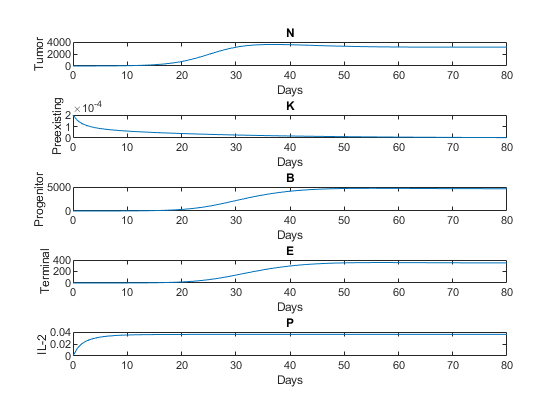
\includegraphics[width=1\textwidth]{pics/Paper_model.png}
    \caption{Reproduction of the homogeneous model dynamics showing the evolution of $N$, $K$, $B$, $E$, and $P$ over time.}
    \label{fig:paper_model}
\end{figure}

\subsection{Extending the model: multiple exhaustion states}
To capture the heterogeneity of T cell exhaustion, the $E$ group of cells has been divided following different levels of exhaustion:
\begin{itemize}
    \item $E_0$: Initially Exhausted T cells (functional, capable of tumor killing).
    \item $E_{1/2}$: Middle-exhausted T cells (partially dysfunctional).
    \item $E_1$: Deeply-exhausted T cells (fully exhausted, negligible killing capabilities).
\end{itemize}
The new model is the following:
\begin{equation}
\begin{cases}
    \dot{N}(t) = \alpha N \left(1 - \frac{N}{T_C}\right) - h \left( \frac{\lambda_k N K + \lambda_0 N E_0 + \lambda_{1/2} N E_{1/2} + \lambda_1 N E_1}{N + K + E_0 + E_{1/2} + E_1} \right), \\[2ex]
    \dot{K}(t) = h P K - \delta_k K, \\[2ex]
    \dot{B}(t) = 2^m S_B N + h P B - r_E B - \delta_B B, \\[2ex]
    \dot{E}_0(t) = r_E B - r_t E_0 - \delta_0 E_0, \\[2ex]
    \dot{E}_{1/2}(t) = r_t E_0 - r_t E_{1/2} - \delta_{1/2} E_{1/2}, \\[2ex]
    \dot{E}_1(t) = r_t E_{1/2} - \delta_1 E_1\\[2ex]
    \dot{P}(t) = \rho_K K + \rho_B B - h P (K + B) - \delta_P P,
\end{cases}
\end{equation}
where:
\begin{itemize}
    \item $\delta_0$, $\delta_{1/2}$, and $\delta_1$ represent the death rates for the initially, middle and deeply exhausted T cells, respectively. Deeper exhaustion is linked with a shorter lifespan, therefore, these rates follow the inequality $\delta_0 < \delta_{1/2} < \delta_1$.
    
    \item $\lambda_0$, $\lambda_{1/2}$, and $\lambda_1$ represent the tumor-killing rates for each corresponding sub-population. Because progressive exhaustion severely affects effector function, the killing capacity decreases as cells transition keep going, leading to $\lambda_0 > \lambda_{1/2} > \lambda_1$.
    
    \item $r_t$ is the phenotypic transition rate, in other words, the speed at which T cells progressively pass from one state to the other in the following order: $E_0 \rightarrow E_{1/2} \rightarrow E_1$.
\end{itemize}
\subsubsection{Equivalence under Homogeneous Assumptions}

First, we demonstrate that if we assume uniform killing and death rates ($\lambda_0 = \lambda_{1/2} = \lambda_1 = \lambda_E$ and $\delta_0 = \delta_{1/2} = \delta_1 = \delta_E$), the extended system turns back to the original model. In fact, if we define the total exhausted population as $E = E_0 + E_{1/2} + E_1$ and substitute the respective differential equations, we can see that:

\begin{equation}
\begin{aligned}
    \dot{E} &= \dot{E}_0 + \dot{E}_{1/2} + \dot{E}_1 \\
    \dot{E} &= (r_E B - r_t E_0 - \delta_E E_0) + (r_t E_0 - r_t E_{1/2} - \delta_E E_{1/2}) + (r_t E_{1/2} - \delta_E E_1) \\
    \dot{E} &= r_E B - \delta_E (E_0 + E_{1/2} + E_1) \\
    \dot{E} &= r_E B - \delta_E E.
\end{aligned}
\end{equation}

By canceling the intermediate transition terms ($r_t E_0$ and $r_t E_{1/2}$), the final result matches exactly the equation for $\dot{E}(t)$ in the original system.
Furthermore, if we conside also the equation for $\dot{N}$, we got:
\begin{equation}
\begin{aligned}
\dot{N} &= \alpha N \left( 1 - \frac{N}{T_C} \right) - h \left( \frac{\lambda_k N K + \lambda_0 N E_0 + \lambda_{1/2} N E_{1/2} + \lambda_1 N E_1}{N + K + E_0 + E_{1/2} + E_1 + 1} \right) & \\
&= \alpha N \left( 1 - \frac{N}{T_C} \right) - h \left( \frac{\lambda_k N K + \lambda_E N E_0 + \lambda_E N E_{1/2} + \lambda_E N E_1}{N + K + E_0 + E_{1/2} + E_1 + 1} \right) & \\
&= \alpha N \left( 1 - \frac{N}{T_C} \right) - h \left( \frac{\lambda_k N K + \lambda_E N (E_0 + E_{1/2} + E_1)}{N + K + (E_0 + E_{1/2} + E_1) + 1} \right) & \\
&= \alpha N \left( 1 - \frac{N}{T_C} \right) - h \left( \frac{\lambda_k N K + \lambda_E N E}{N + K + E + 1} \right) &
\end{aligned}
\end{equation}
confirming that, with homogeneous assumptions, the model obtained is again the original one. This equivalence is validated numerically below.
\begin{figure}[H]
    \centering
    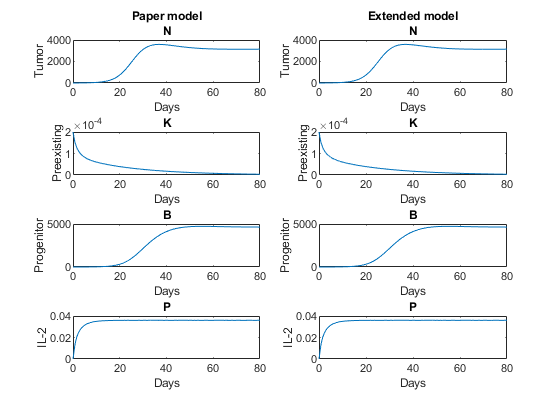
\includegraphics[width=0.8\textwidth]{pics/PapervsNewHomo.png}
    \caption{Comparison between the original system and the new one with $r_t=5r_E$}
\end{figure}

\begin{figure}[H]
    \centering
    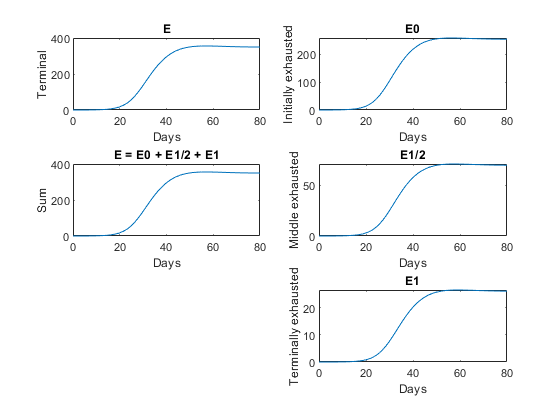
\includegraphics[width=0.8\textwidth]{pics/E_sum_rt5.png}
    \caption{Comparison with $r_t=5r_E$ showing that the sum of the extended compartments ($E_0 + E_{1/2} + E_1$) perfectly overlaps with the $E$ compartment from the homogeneous paper model.}
\end{figure}

\begin{figure}[H]
    \centering
    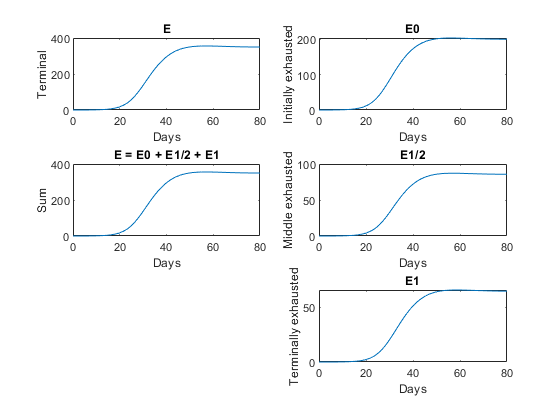
\includegraphics[width=0.8\textwidth]{pics/E_sum_rt10.png}
    \caption{Comparison with $r_t=10r_E$ showing that the sum of the extended compartments ($E_0 + E_{1/2} + E_1$) perfectly overlaps with the $E$ compartment from the homogeneous paper model.}
\end{figure}

It is good to notice that while the sum $E_0 + E_{1/2} + E_1$ remains the the same with both values of $r_t$, the composition of the sum is different: 

\begin{itemize}
    \item When $r_t$ is lower ($r_t = 5r_E$, Figure 3), the transition is slower, causing most cells to remain in an initial exhaustion state ($E_0$).
    \item When $r_t$ is doubled ($r_t = 10r_E$, Figure 4), cells become exhausted much faster. As a result, the peak $E_0$ population drops, while the deeply exhausted groups ($E_{1/2}$ and $E_1$) grow more.
\end{itemize}

\subsubsection{Introduction of heterogeneity in killing and death rates}
Deeply exhausted T cells have shorter lifespans and lower tumor-killing capacities. To simulate that, we define a continuous linear function for the killing rate $\lambda(y)$ and death rate $\delta(y)$ as functions of $y \in [0,1]$:
$$ \lambda(y) = \lambda_K + y(\lambda_E - \lambda_K) $$
$$ \delta(y) = \delta_K + y(\delta_E - \delta_K) $$
Using these linear functions, we evaluate the intermediate state ($y=1/2$) to derive $\lambda_{1/2}$ and $\delta_{1/2}$:
$$ \lambda_{1/2} = \lambda_K + \frac{1}{2}(\lambda_E - \lambda_K) $$
$$ \delta_{1/2} = \delta_K + \frac{1}{2}(\delta_E - \delta_K) $$
With this choice, we assumed that Initially Exhausted T cells ($y=0$) have the same killing/death rate as Healthy T cells and that Deeply Exhausted T cells  ($y=1$) have the same killing/death rate as the Terminally T cells.

\subsection{Simulation and Analysis of the Extended Model}
The implementation of these heterogeneous rates modify the dynamics of the tumor-immune interaction, as shown below.

\begin{figure}[H]
    \centering
    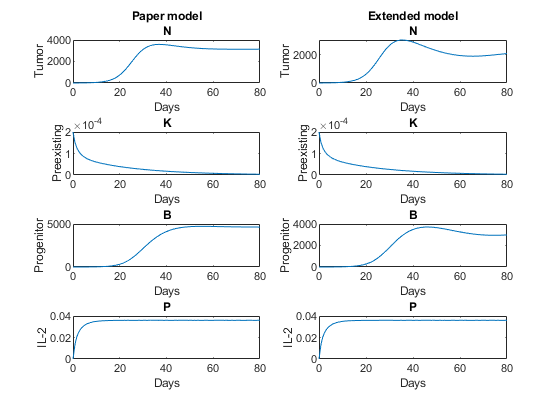
\includegraphics[width=0.8\textwidth]{pics/PapervsNewHet.png}
    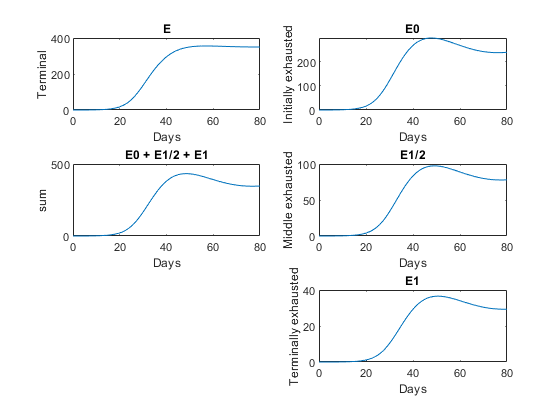
\includegraphics[width=0.8\textwidth]{pics/E_sum_rt5_Het.png}
    \caption{Evolution of variables under heterogeneous assumptions compared to the original systemwith $r_t =5\cdot r_E$.}
\end{figure}

By adding specific death and killing rates based on how exhausted the cells are, the early exhausted cells ($E_0$) provide a strong, immediate killing power that is similar to fully functional CTLs. However, because these cells transform into deeply exhausted cells ($E_1$) and have higher death rates, the size and stability of the tumor-immune balance changes. 

Specifically, the strong early attack from $E_0$ causes a sharp drop in tumor size. This creates a new balance at a much lower tumor level than what the homogeneous model predicts. This drop causes a major "domino" effect on the other cell types. Because the presence of Progenitor cells ($B$) depends directly on the tumor size through the developmental program term $2^m s_B N$, a smaller tumor means less antigen stimulation. 

Consequently, the Progenitor population ($B$) reaches a peak and then drops to a lower steady state than in the homogeneous model. This smaller supply limits the growth of $E_0$. As a result, fewer cells move on to the later $E_{1/2}$ and $E_1$ stages. This explains why the total number of exhausted cells ($E_0 + E_{1/2} + E_1$) drops to a lower balance after its first highly effective spike.

In conclusion, having more functional cells ($E_0$) clears the tumor faster. However, by removing the constant antigen stimulation, the immune system cuts off its own supply of T cells, resulting in a permanent stalemate.

\section{Continuous Population Model}
Biological phenomena involving phenotypic variation can often be more accurately modeled as continuous spectra rather than discrete compartments. In this section we will formulate an extension of the model introducing a continuous phenotype $y \in [0,1]$. We will define $E(t,y)$ as a density function representing the total number of exhausted cells at time $t$ characterized by phenotype $y$, governed by a Partial Differential Equation.

\subsection{Derivation of the model}

We want to distinguish exhausted cells based on their exhaustion level, represented by a continuous phenotype variable $y \in [0,1]$. To model how the characteristics of these cells change as they become more exhausted, we define the tumor-killing parameter $\lambda_t(y)$ and the death rate $\delta_t(y)$ as functions of the phenotype $y$:

\begin{equation}
\begin{aligned}
\lambda_t(y) &= \lambda_K + y(\lambda_E - \lambda_K) \\ 
\delta_t(y) &= \delta_K + y(\delta_E - \delta_K).
\end{aligned}
\end{equation}
\\
Starting from the original model equation:

\begin{equation}
\begin{aligned}
\frac{dE_{tot}(t)}{dt} = r_E B(t) - \delta_E E_{tot}(t) \\
\end{aligned}
\end{equation}

we define a density function $E(t,y)$ such that the total number of cells is expressed by:

\begin{equation}
\begin{aligned}
E_{tot}(t)=\int^1_0 E(t,y)dy.\\
\end{aligned}
\end{equation}

If we consider a small piece of the space $\Delta y$ at time $t$, we have that the number of cells in this piece is defined by:
\begin{itemize}
    \item number of still functional cells,
    \item number of cells that mutate towards exhaustion,
    \item number of dying cells, regulated by $\delta_t(y)$.
\end{itemize}

Introducing $v(t,y)$ as the cells aging speed, the equation becomes:

\begin{equation}
\begin{aligned}
\frac{\partial}{\partial t}[E(t,y) \Delta y] = v(t,y)E(t,y)-v(t,y+\Delta y)E(t,y+\Delta y)-\delta_t(y) E(t,y)\Delta y \\
\end{aligned}
\end{equation}
and dividing by $\Delta y$, we obtain the incremental ratio:

\begin{equation}
\begin{aligned}
\frac{\partial}{\partial t}E(t,y)= \frac{v(t,y)E(t,y)-v(t,y+\Delta y)E(t,y+\Delta y)}{\Delta y}-\delta_t(y) E(t,y). \\
\end{aligned}
\end{equation}

Taking the limit $\Delta y\rightarrow0$, we obtain:

\begin{equation}
\begin{aligned}
\frac{\partial}{\partial t}E(t,y)= -\frac{\partial}{\partial y}(v(t,y)E(t,y))-\delta_t(y) E(t,y) \\
\end{aligned}
\end{equation}
rearranging the terms, we recognize an advection-reaction PDE:

\begin{equation}
\begin{aligned}
\frac{\partial}{\partial t}E(t,y) +\frac{\partial}{\partial y}(v(t,y)E(t,y))=-\delta_t(y) E(t,y). \\
\end{aligned}
\end{equation}

To have a unique solution we have to put some boundary conditions, and we choose them in order to respect the initial equation: at the beginning of exhaustion, we know that the exhausted cells come from the term $r_E B(t)$, that we can consider as the incoming flux on the left side, i.e. 
\begin{equation}
\begin{aligned}
v(t,0)E(t,0)=r_E B(t).
\end{aligned}
\end{equation}

The final system of ODEs and PDEs is the following:

\begin{equation}
\begin{cases}
    \dot{N}(t) = \alpha N \left(1 - \frac{N}{T_c}\right) - h \left( \frac{\lambda_K N K + N\int_0^1\lambda_t(y)E(t,y)dy}{N + K + E_{tot} + 1} \right) \\[2ex]
    \dot{K}(t) = h P K - \delta_K K \\[2ex]
    \dot{B}(t) = 2^m s_B N + h P B - r_E B - \delta_B B \\[2ex]
    \dot{P}(t) = \rho_K K + \rho_B B - h P (K + B) - \delta_P P\\[2ex]
    \frac{\partial E(t,y) }{\partial t}= -\frac{\partial}{\partial y}(v(t,y)E(t,y))-\delta_t(y) E(t,y) \\[2ex]
    %v(t,0)
    v(t,0)E(t,0)=r_E B(t)
\end{cases}
\end{equation}

\subsection{Numerical approach}

To numerically solve the coupled system of ordinary and partial differential equations (ODEs and PDEs), we used the Method of Lines (MOL). This technique allows to decouple the spatial and temporal discretizations: the continuous phenotype domain, $y \in [0, 1]$, is partitioned into an evenly spaced grid of $r = 1001$ nodes with a constant spatial step size $h$. Consequently, the PDE governing the density of exhausted cells, $E(t,y)$, is transformed into a system of $r$ interconnected ODEs.

To discretize the space, we use a first-order backward finite difference approximation (upwind scheme) for the advection term:

\begin{equation}
    \frac{d}{dt}E_i = \frac{v_{i-1}E_{i-1} - v_iE_i}{h} - \delta_i E_i \quad \text{for } i = 1, \dots, r
\end{equation}

This is because cells travel in only one direction in the phenotype space, meaning that cells can only go towards exhaustion and cannot ``heal'' and reverse the aging process. The reaction term, which represents the phenotype dependent death rate $\delta_t(y)E(t,y)$, is calculated directly at each point on the grid. This turns the PDE into a sparse matrix, $A_{PDE}$, where the advection and reaction values are on the main diagonal and the subdiagonal below. 

Furthermore, the boundary condition $v(t,0)E(t,0)=r_EB(t)$ representing progenitor cells turning into initially exhausted cells is added by linking the $B(t)$ variable to the first point of the grid:

\begin{equation}
    \frac{d}{dt}E_1 = \frac{\left[r_EB(t)\right] - v_1E_1}{h} - \delta_1E_1
\end{equation}

In our numerical model, the state vector is organized as $X = [N, K, B, P, E_1, \dots, E_r]^T$. To correctly align the $A_{PDE}$ matrix with this full state vector, we add $r \times 4$ columns of zeros to its left side. This makes sure that the discrete PDE only interacts with the correct macroscopic variables. Specifically, the boundary input term is placed in the first row and third column of $A_{PDE}$. This matches the exact position of the progenitor cells variable $B(t)$:

\begin{equation}
     A_{PDE}(1, 3) = r_E/h.
\end{equation}

Because the system has many equations ($4 + r$) and involves different time scales, the resulting ODE system becomes very stiff. To solve this, we calculate the time integration using MATLAB's \texttt{ode15s} solver. This tool is optimized for stiff problems and is based on Numerical Differentiation Formulas (NDF). To make the simulation faster, we provided the solver with the sparse Jacobian matrix $J$:

\begin{equation}
    J = \begin{bmatrix}
        A_{ODE} \\
        A_{PDE}
    \end{bmatrix}
\end{equation}

In this matrix, the top block $A_{ODE} \in \mathbb{R}^{4 \times (4+r)}$ describes the nonlinear interactions between the main variables ($N$, $K$, $B$, $P$) and the total exhausted population. The bottom block $A_{PDE} \in \mathbb{R}^{r \times (4+r)}$ contains the dynamics of the exhaustion process, including the boundary condition. The overall structure of the Jacobian matrix can be seen below:

\begin{equation}
J = \left[
\begin{array}{cccc|ccccc}
\frac{\partial \dot{N}}{\partial N} & \frac{\partial \dot{N}}{\partial K} & 0 & 0 & \frac{\partial \dot{N}}{\partial E_1} & \cdots & \frac{\partial \dot{N}}{\partial E_j} & \cdots & \frac{\partial \dot{N}}{\partial E_r} \\[2ex]
0 & \frac{\partial \dot{K}}{\partial K} & 0 & \frac{\partial \dot{K}}{\partial P} & 0 & \cdots & 0 & \cdots & 0 \\[2ex]
\frac{\partial \dot{B}}{\partial N} & 0 & \frac{\partial \dot{B}}{\partial B} & \frac{\partial \dot{B}}{\partial P} & 0 & \cdots & 0 & \cdots & 0 \\[2ex]
0 & \frac{\partial \dot{P}}{\partial K} & \frac{\partial \dot{P}}{\partial B} & \frac{\partial \dot{P}}{\partial P} & 0 & \cdots & 0 & \cdots & 0 \\[2ex]
\hline
0 & 0 & \frac{r_E}{h} & 0 & -\left(\frac{v_1}{h}+\delta_1\right) & 0 & \cdots & \cdots & 0 \\[2ex]
0 & 0 & 0 & 0 & \frac{v_1}{h} & -\left(\frac{v_2}{h}+\delta_2\right) & \ddots & & \vdots \\[2ex]
\vdots & \vdots & \vdots & \vdots & 0 & \ddots & \ddots & \ddots & \vdots \\[2ex]
\vdots & \vdots & \vdots & \vdots & \vdots & \ddots & \frac{v_{r-2}}{h} & -\left(\frac{v_{r-1}}{h}+\delta_{r-1}\right) & 0 \\[2ex]
0 & 0 & 0 & 0 & 0 & \cdots & 0 & \frac{v_{r-1}}{h} & -\left(\frac{v_r}{h}+\delta_r\right)
\end{array}
\right]
\end{equation}

\subsection{Results and discussion}

Numerical results are presented below: as we can see, 

\begin{figure}[H]
    \centering
    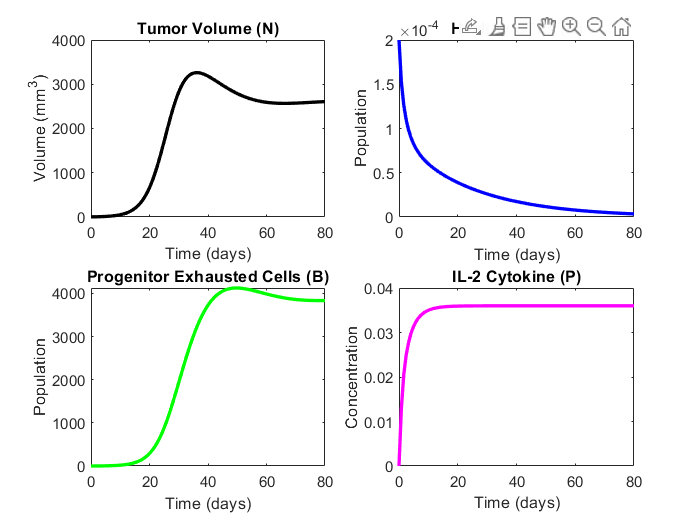
\includegraphics[width=0.8\textwidth]{pics/ODEs.png}
    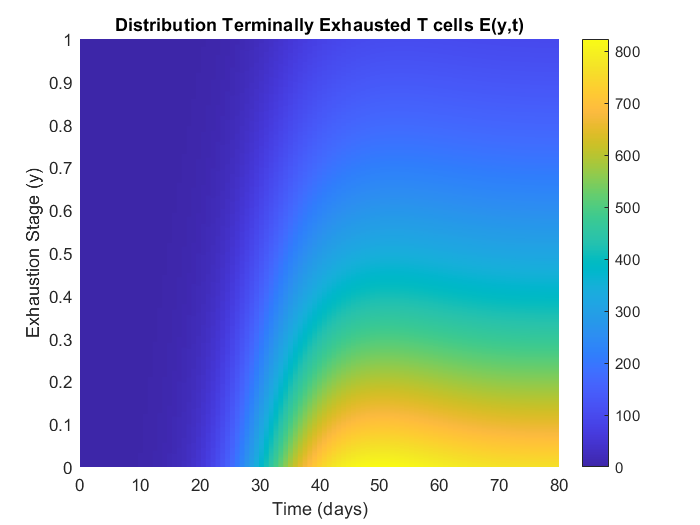
\includegraphics[width=0.8\textwidth]{pics/heatmap.png}
    \caption{Evolution of variables under heterogeneous assumptions compared to the original system with $r_t =5\cdot r_E$.}
    \label{fig:hetero_dyn}
\end{figure}

\subsection{Conclusions}



\newpage
\bibliographystyle{plain}
\nocite{*}
\bibliography{ref.bib}
\end{document}